\title{Assignment 1 \\ \small{Evolutionary Computing}}
\author{Chiel ten Brinke 3677133}
\documentclass[12pt]{article}
\usepackage{amssymb,amsmath,amsthm,enumerate,graphicx,float,lmodern,xparse}

\newtheorem{theorem}{Theorem}[section]
\newtheorem{lemma}[theorem]{Lemma}
\newtheorem{proposition}[theorem]{Proposition}
\newtheorem{corollary}[theorem]{Corollary}

\theoremstyle{definition}
\newtheorem{definition}[theorem]{Definition}
\newtheorem{axiom}[theorem]{Axiom}
\newtheorem{example}[theorem]{Example}
\newtheorem{remark}[theorem]{Remark}

\NewDocumentCommand\set{mg}{%
    \ensuremath{\left\lbrace #1 \IfNoValueTF{#2}{}{\, \middle|\, #2} \right\rbrace}%
}

\begin{document}
\maketitle

\section*{Results}

\subsection*{Experiment 1}

\subsubsection*{Counting ones}
%Required population size: 310
%Function evaluations: 51094
%Corresponding cumulative CPU time: 0.013 seconds
\begin{table}[H]
\begin{tabular}{|ll|}
\hline
\textbf{Required population size} & 310              \\ \hline
\textbf{Function evaluations}     & 51094            \\ \hline
\textbf{Corresponding CPU time}   & 0.013 seconds    \\ \hline
\end{tabular}
\end{table}


\subsubsection*{Linearly scaled counting ones}
%Required population size: 730
%Function evaluations: 164174
%Corresponding cumulative CPU time: 0.030 seconds
\begin{table}[H]
\begin{tabular}{|ll|}
\hline
\textbf{Required population size} & 730              \\ \hline
\textbf{Function evaluations}     & 164174            \\ \hline
\textbf{Corresponding CPU time}   & 0.030 seconds    \\ \hline
\end{tabular}
\end{table}

\subsubsection*{Tightly linked deceptive trap}
%Required population size: 1210
%Function evaluations: 243142
%Corresponding cumulative CPU time: 0.429 seconds
\begin{table}[H]
\begin{tabular}{|ll|}
\hline
\textbf{Required population size} & 1210              \\ \hline
\textbf{Function evaluations}     & 243142            \\ \hline
\textbf{Corresponding CPU time}   & 0.429 seconds    \\ \hline
\end{tabular}
\end{table}

\subsubsection*{Tightly linked non-deceptive trap}
%Required population size: 610
%Function evaluations: 93278
%Corresponding cumulative CPU time: 0.177 seconds
\begin{table}[H]
\begin{tabular}{|ll|}
\hline
\textbf{Required population size} & 610              \\ \hline
\textbf{Function evaluations}     & 93278            \\ \hline
\textbf{Corresponding CPU time}   & 0.177 seconds    \\ \hline
\end{tabular}
\end{table}


\begin{figure}[H]
    \centering
    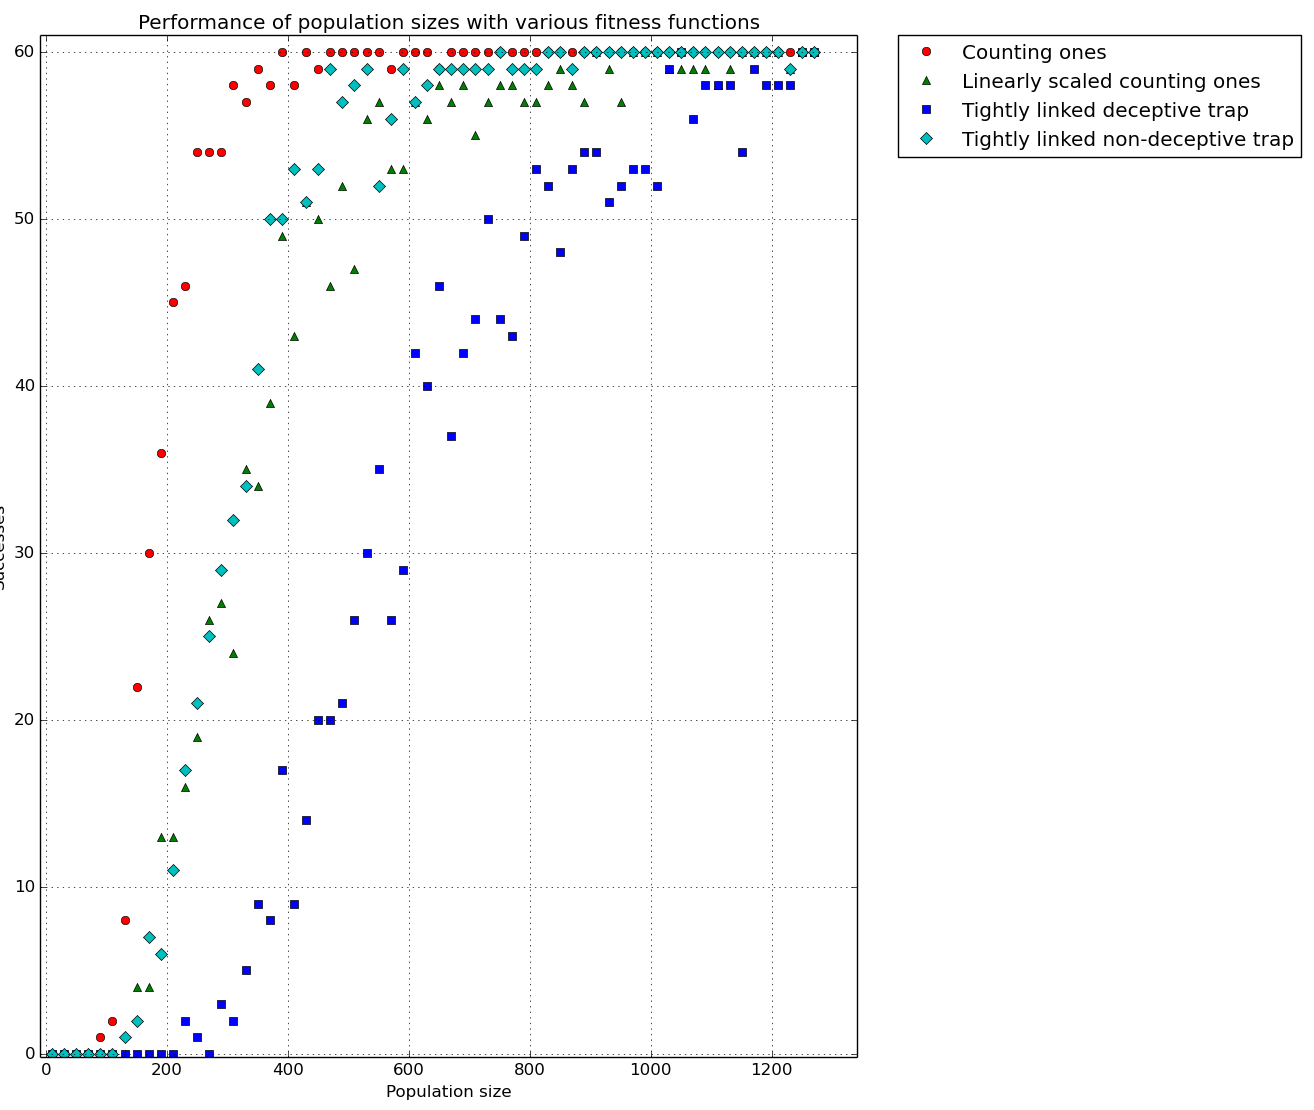
\includegraphics[width=1\linewidth]{images/exp1.png}
    \caption{TODO}
\label{fig:exp1}
\end{figure}


\subsection*{Experiment 2}
\begin{figure}[H]
    \centering
    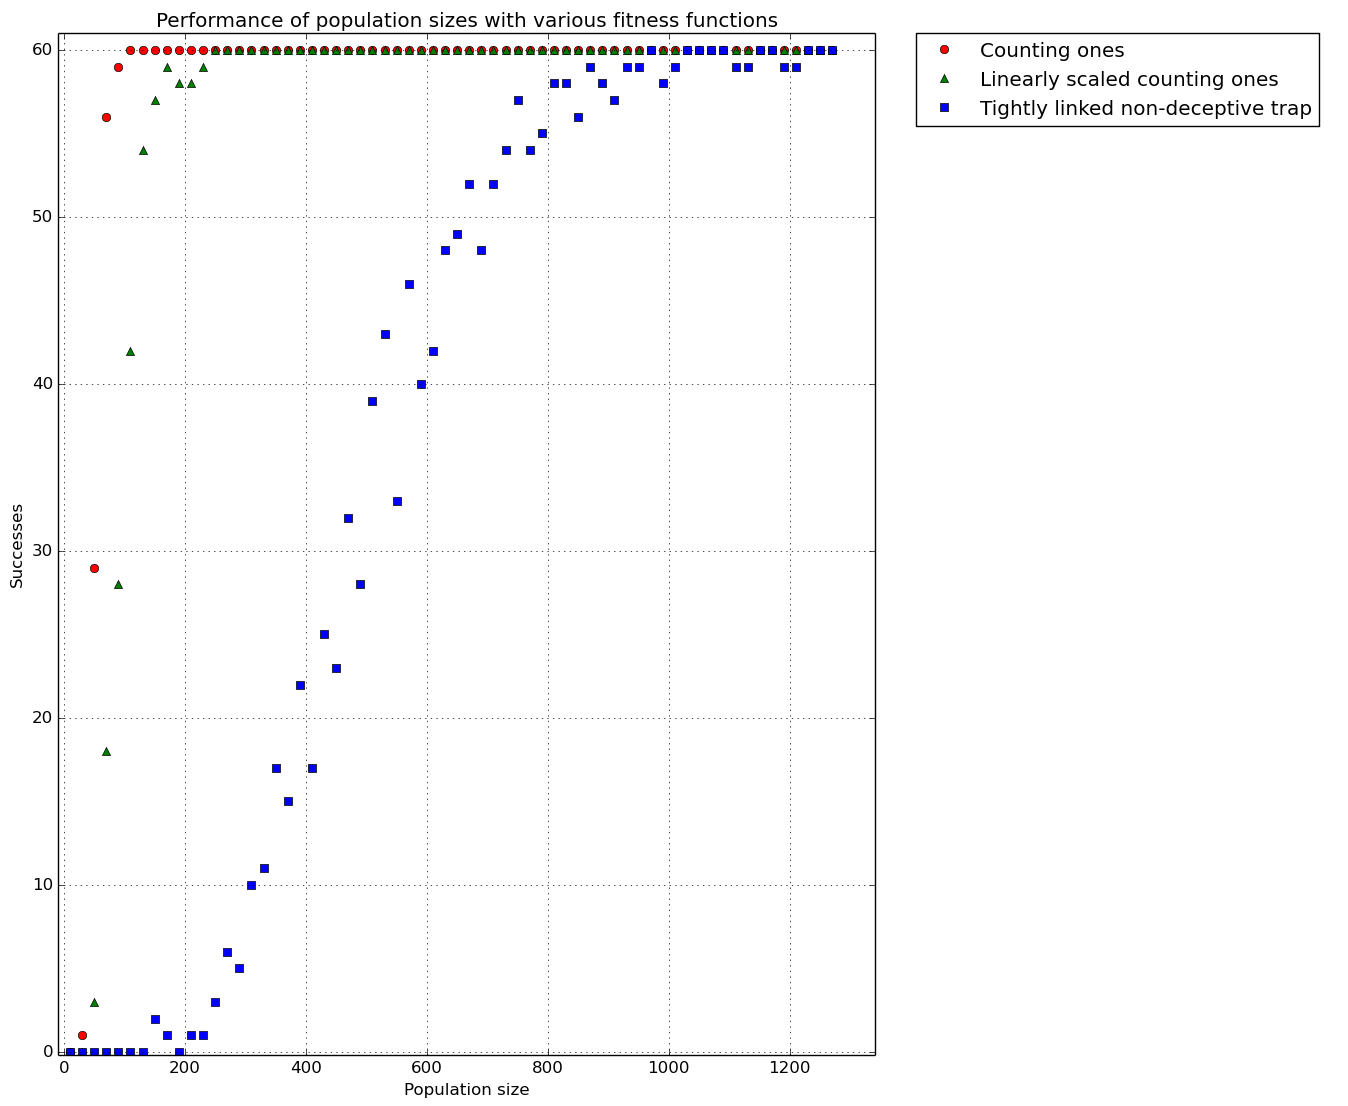
\includegraphics[width=1\linewidth]{images/exp2.png}
    \caption{TODO}
\label{fig:exp2}
\end{figure}


\subsection*{Experiment 3}
\begin{figure}[H]
    \centering
    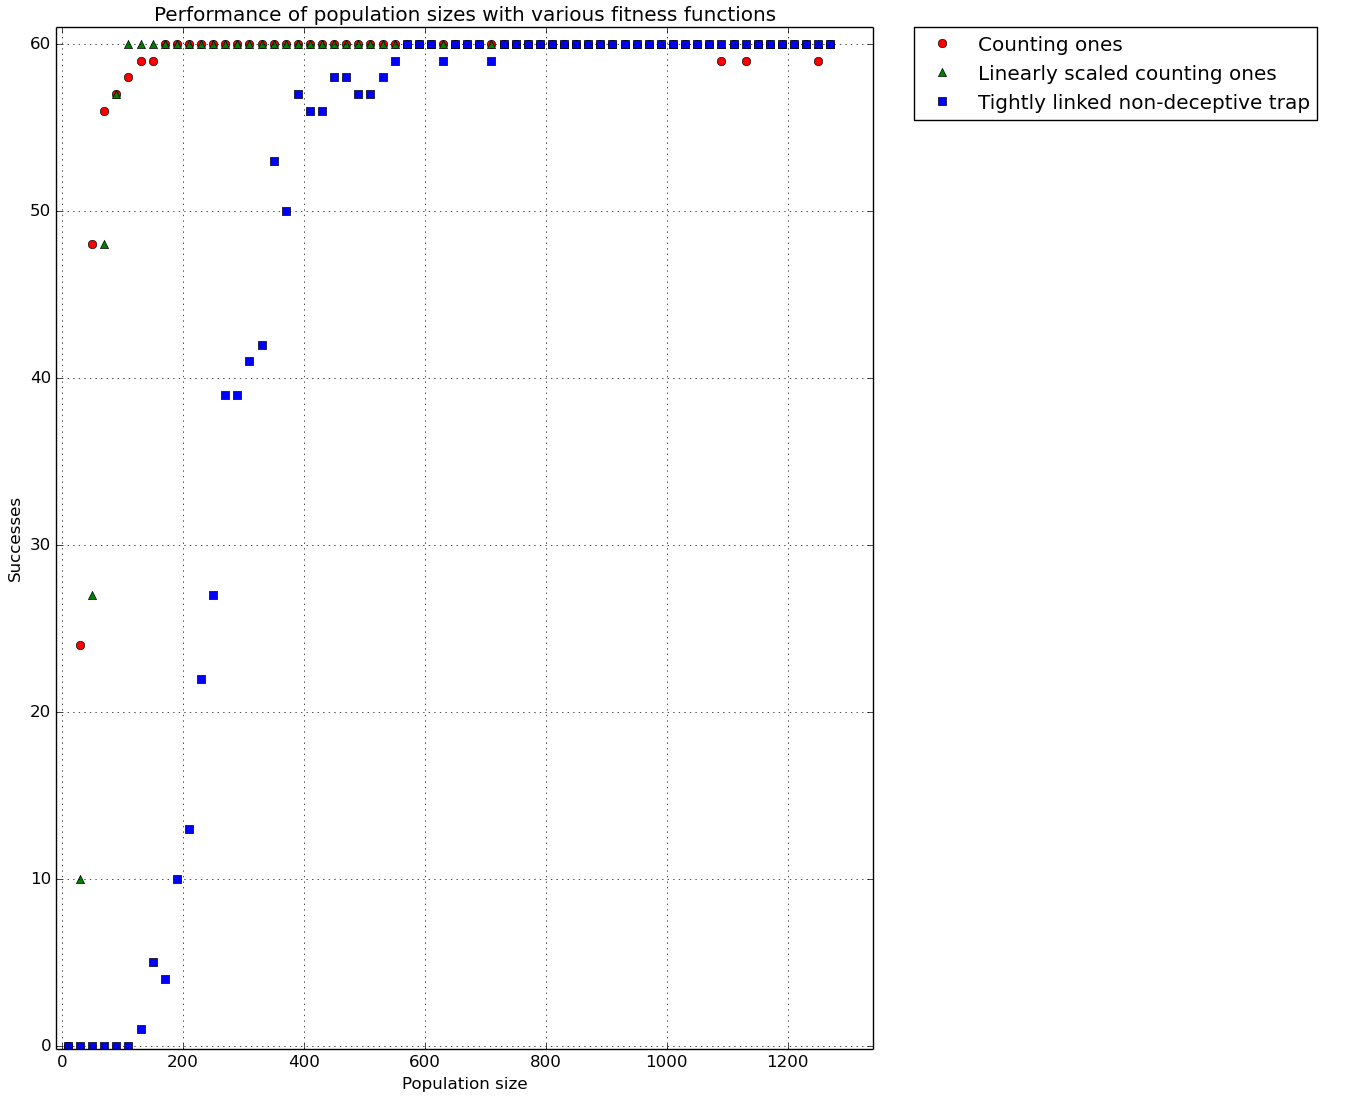
\includegraphics[width=1\linewidth]{images/exp3.png}
    \caption{TODO}
\label{fig:exp3}
\end{figure}

\end{document}
